
\documentclass[twoside,11pt]{homework}
\usepackage{graphicx}
\usepackage{listings}
\usepackage{color}
\usepackage{bm}
\newcommand{\vect}[1]{\boldsymbol{\mathbf{#1}}}
\definecolor{dkgreen}{rgb}{0,0.6,0}
\definecolor{gray}{rgb}{0.5,0.5,0.5}
\definecolor{mauve}{rgb}{0.58,0,0.82}
\lstset{ %
	language=R,                     % the language of the code
	basicstyle=\footnotesize,       % the size of the fonts that are used for the code
	numbers=left,                   % where to put the line-numbers
	numberstyle=\tiny\color{gray},  % the style that is used for the line-numbers
	stepnumber=1,                   % the step between two line-numbers. If it's 1, each line
	% will be numbered
	numbersep=5pt,                  % how far the line-numbers are from the code
	backgroundcolor=\color{white},  % choose the background color. You must add \usepackage{color}
	showspaces=false,               % show spaces adding particular underscores
	showstringspaces=false,         % underline spaces within strings
	showtabs=false,                 % show tabs within strings adding particular underscores
	frame=single,                   % adds a frame around the code
	rulecolor=\color{black},        % if not set, the frame-color may be changed on line-breaks within not-black text (e.g. commens (green here))
	tabsize=2,                      % sets default tabsize to 2 spaces
	captionpos=b,                   % sets the caption-position to bottom
	breaklines=true,                % sets automatic line breaking
	breakatwhitespace=false,        % sets if automatic breaks should only happen at whitespace
	title=\lstname,                 % show the filename of files included with \lstinputlisting;
	% also try caption instead of title
	keywordstyle=\color{blue},      % keyword style
	commentstyle=\color{dkgreen},   % comment style
	stringstyle=\color{mauve},      % string literal style
	escapeinside={\%*}{*)},         % if you want to add a comment within your code
	morekeywords={*,...},            % if you want to add more keywords to the set
	belowcaptionskip=0em,
	belowskip=0em
} 

\usepackage{etoolbox}
\makeatletter
\patchcmd{\@verbatim}
{\verbatim@font}
{\verbatim@font\footnotesize}
{}{}
\preto{\@verbatim}{\topsep=0pt \partopsep=0pt }
\makeatother

\coursename{COMS 4771 Machine Learning } % DON'T CHANGE THIS

\studname{Jun Hu}    % YOUR NAME GOES HERE
\studmail{jh3846@columbia.edu}% YOUR UNI GOES HERE
\hwNo{2}                   % THE HOMEWORK NUMBER GOES HERE
\collab{}   % THE UNI'S OF STUDENTS YOU DISCUSSED WITH

% Uncomment the next line if you want to use \includegraphics.\textbf{\textbf{\textbf{}}}
%\usepackage{graphicx}

\begin{document}
\maketitle

\section*{Problem 1}

\begin{enumerate}
\item[\textbf{(a)}] Execute:

\begin{lstlisting}
library(tree)
library(ISLR)
set.seed(2388)
train = sample(1:nrow(OJ), 800)
OJ.train = OJ[train, ]
OJ.test = OJ[-train, ]
\end{lstlisting}

\item[\textbf{(b)}] Fit and summarize:

\begin{lstlisting}
tree.oj = tree(Purchase~., data=OJ.train)
summary(tree.oj)
\end{lstlisting}

Will return:

\begin{verbatim}
Classification tree:
tree(formula = Purchase ~ ., data = OJ.train)
Variables actually used in tree construction:
[1] "LoyalCH"       "PriceDiff"     "StoreID"       "ListPriceDiff" "PctDiscMM"    
Number of terminal nodes:  10 
Residual mean deviance:  0.7451 = 588.6 / 790 
Misclassification error rate: 0.1662 = 133 / 800

\end{verbatim}

From the results, we can obtain that the classification tree actually uses only 5 variables, which are LoyalCH, PriceDiff, StoreID, ListPriceDiff, PctDiscMM. The tree has 10 terminal nodes, and the misclassification error rate is 0.1662.

\item[\textbf{(c)}] Execute:

\begin{lstlisting}
tree.oj
\end{lstlisting}

\begin{verbatim}
node), split, n, deviance, yval, (yprob)
      * denotes terminal node

 1) root 800 1072.00 CH ( 0.60750 0.39250 )  
   2) LoyalCH < 0.5036 349  418.10 MM ( 0.28653 0.71347 )  
     4) LoyalCH < 0.282272 174  135.90 MM ( 0.13218 0.86782 )  
       8) LoyalCH < 0.0356415 56   10.03 MM ( 0.01786 0.98214 ) *
       9) LoyalCH > 0.0356415 118  113.50 MM ( 0.18644 0.81356 ) *
     5) LoyalCH > 0.282272 175  240.10 MM ( 0.44000 0.56000 )  
      10) PriceDiff < 0.05 70   72.74 MM ( 0.21429 0.78571 )  
        20) StoreID < 1.5 19    0.00 MM ( 0.00000 1.00000 ) *
        21) StoreID > 1.5 51   61.79 MM ( 0.29412 0.70588 ) *
      11) PriceDiff > 0.05 105  142.10 CH ( 0.59048 0.40952 )  
        22) LoyalCH < 0.482304 75  104.00 MM ( 0.49333 0.50667 ) *
        23) LoyalCH > 0.482304 30   27.03 CH ( 0.83333 0.16667 ) *
   3) LoyalCH > 0.5036 451  372.00 CH ( 0.85588 0.14412 )  
     6) LoyalCH < 0.764572 192  228.10 CH ( 0.71875 0.28125 )  
      12) ListPriceDiff < 0.235 74  102.40 MM ( 0.47297 0.52703 )  
        24) PctDiscMM < 0.196196 58   79.30 CH ( 0.56897 0.43103 ) *
        25) PctDiscMM > 0.196196 16   12.06 MM ( 0.12500 0.87500 ) *
      13) ListPriceDiff > 0.235 118   89.89 CH ( 0.87288 0.12712 ) *
     7) LoyalCH > 0.764572 259   91.02 CH ( 0.95753 0.04247 ) *
     
\end{verbatim}

Let's pick the terminal node (marked with *) labeled as 8). It shows that the split criterion is LoyalCH $<$ 0.0356415, the number of observations in this branch is 56, the deviance is 10.03, the overall prediction for the branch is MM for Purchase, and $98.214\%$ observations in this branch is MM for Purchase while $1.786\%$ is CH for Purchase.

\item[\textbf{(d)}] Execute:

\begin{lstlisting}
plot(tree.oj)
text(tree.oj, pretty=0)
\end{lstlisting}

The plot is:

\begin{center}
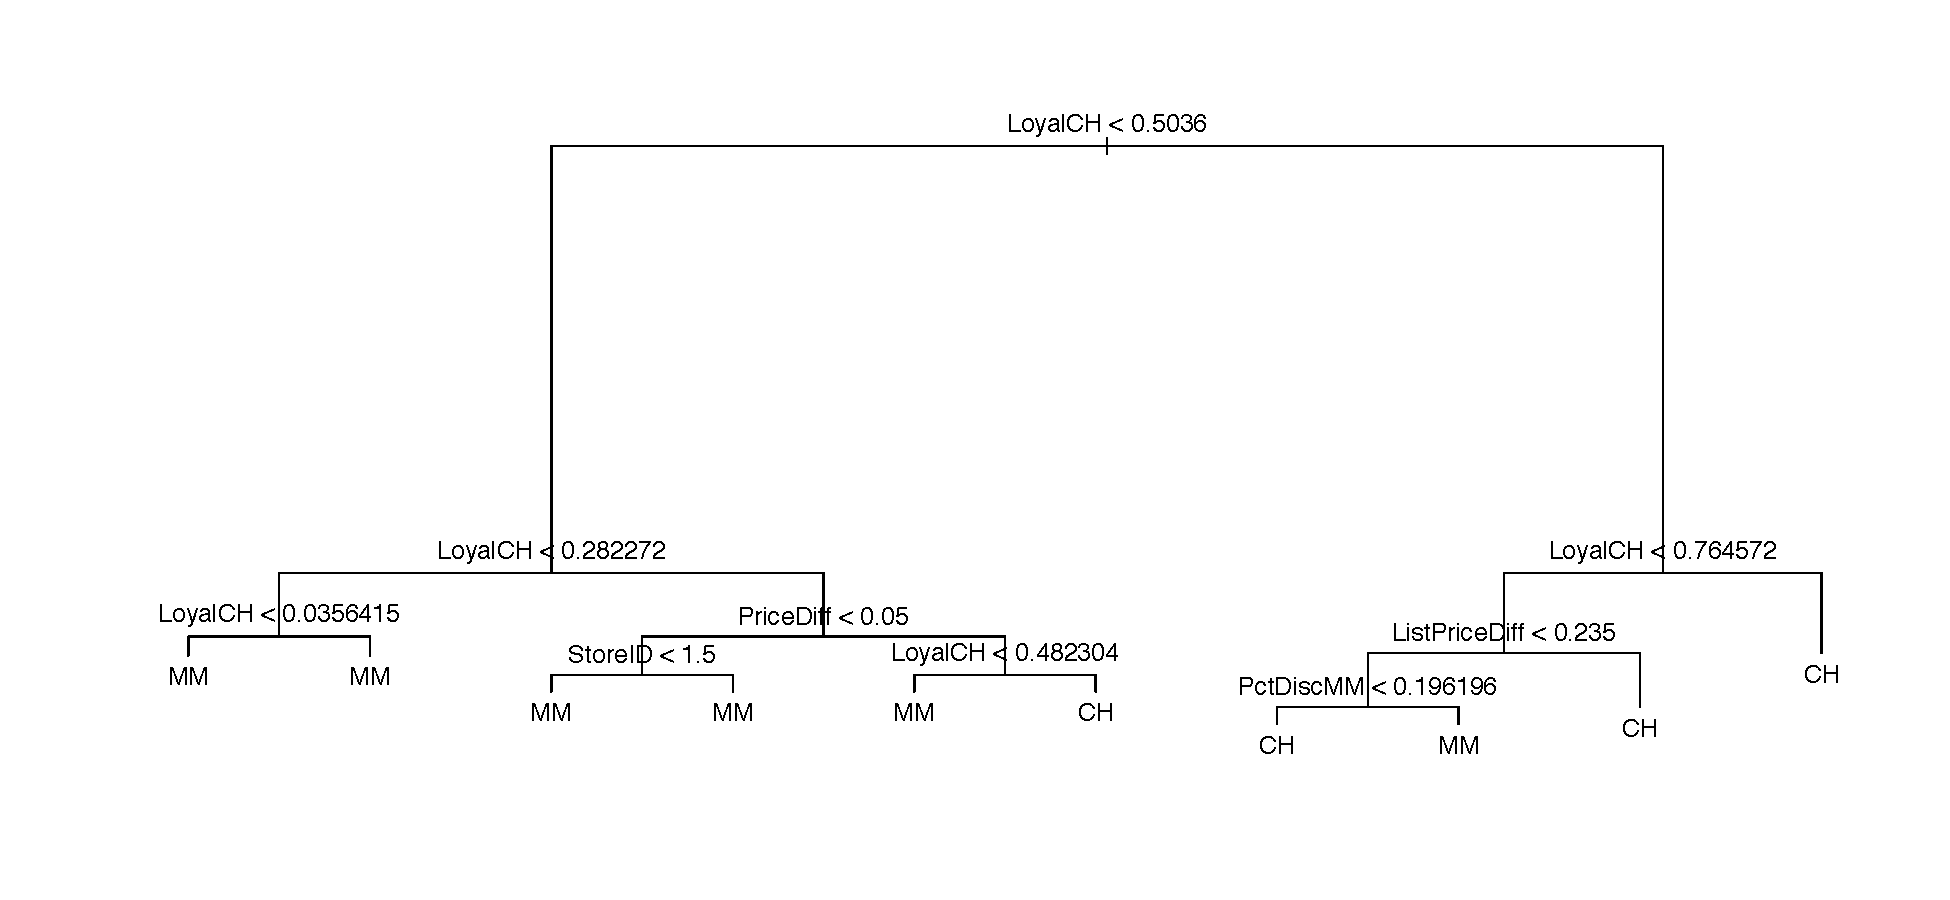
\includegraphics[height=0.31\textheight]{g1.pdf}
\end{center}

This plot indicates the importance of the variable LoyalCH. Because the first level split criterion is LoyalCH $\lessgtr$ 0.5036, then in the second level the two nodes still splits on LoyalCH (LoyalCH $\lessgtr$ 0.282272, LoyalCH $\lessgtr$ 0.764572).

\item[\textbf{(e)}] Execute:

Predict and produce a confusion matrix:

\begin{lstlisting}
tree.pred = predict(tree.oj, OJ.test, type="class")
table(tree.pred, OJ.test$Purchase)
\end{lstlisting}

\begin{verbatim}
tree.pred  CH  MM
       CH 141  17
       MM  26  86
       
\end{verbatim}

Calculate the test error rate:

\begin{lstlisting}
mean(tree.pred!=OJ.test$Purchase)
\end{lstlisting}

\begin{verbatim}
[1] 0.1592593

\end{verbatim}

So the test error rate is $15.93\%$.

\item[\textbf{(f)}] Execute cv.tree function as:

\begin{lstlisting}
cv.oj = cv.tree(tree.oj, FUN=prune.misclass)
\end{lstlisting}

Check results:

\begin{lstlisting}
cv.oj
\end{lstlisting}

\begin{verbatim}
$size
[1] 10  8  7  4  2  1

$dev
[1] 163 163 165 161 174 314

$k
[1]  -Inf   0.0   1.0   4.0   9.5 149.0

$method
[1] "misclass"

attr(,"class")
[1] "prune"         "tree.sequence"

\end{verbatim}

\item[\textbf{(g)}] Plot as:

\begin{lstlisting}
plot(cv.oj$size, cv.oj$dev, type='b', col="red", ylim=c(160, 315), lwd=3, xlab='size', ylab='cross-validated classification error rate')
\end{lstlisting}

\begin{center}
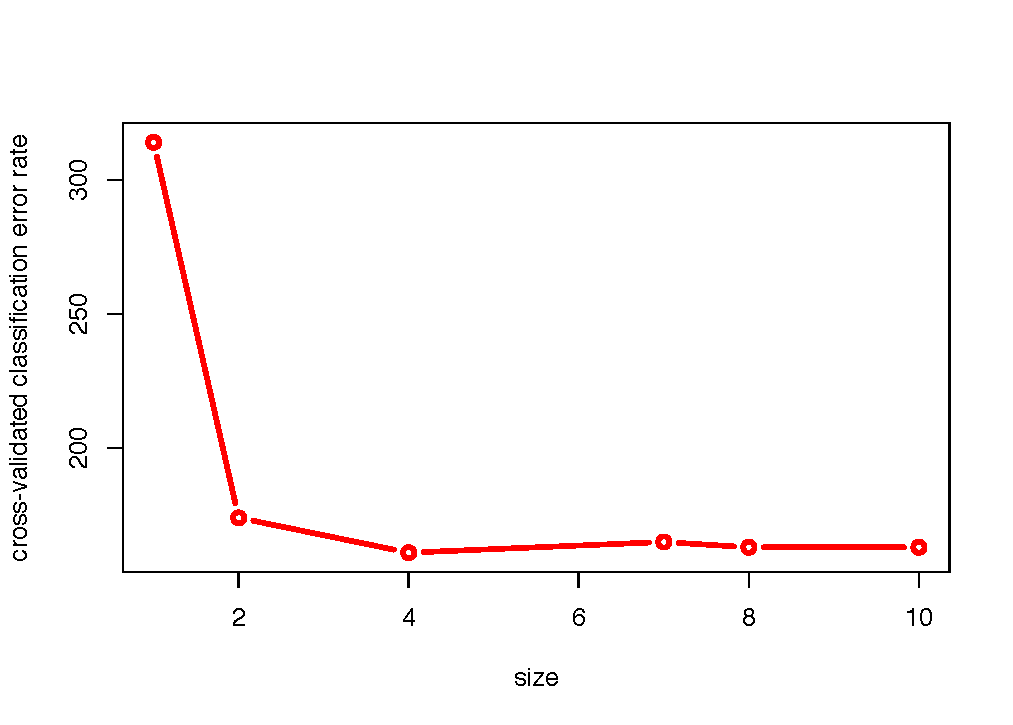
\includegraphics[height=0.35\textheight]{g2.pdf}
\end{center}


\item[\textbf{(h)}] From \textbf{(f)} and \textbf{(g)} we can get the tree size of $4$ returns the lowest cross-validated classification error rate.

\item[\textbf{(i)}] Prune the tree as:

\begin{lstlisting}
prune.oj = prune.misclass(tree.oj, best=4)
plot(prune.oj)
text(prune.oj, pretty=0)
\end{lstlisting}

\begin{center}
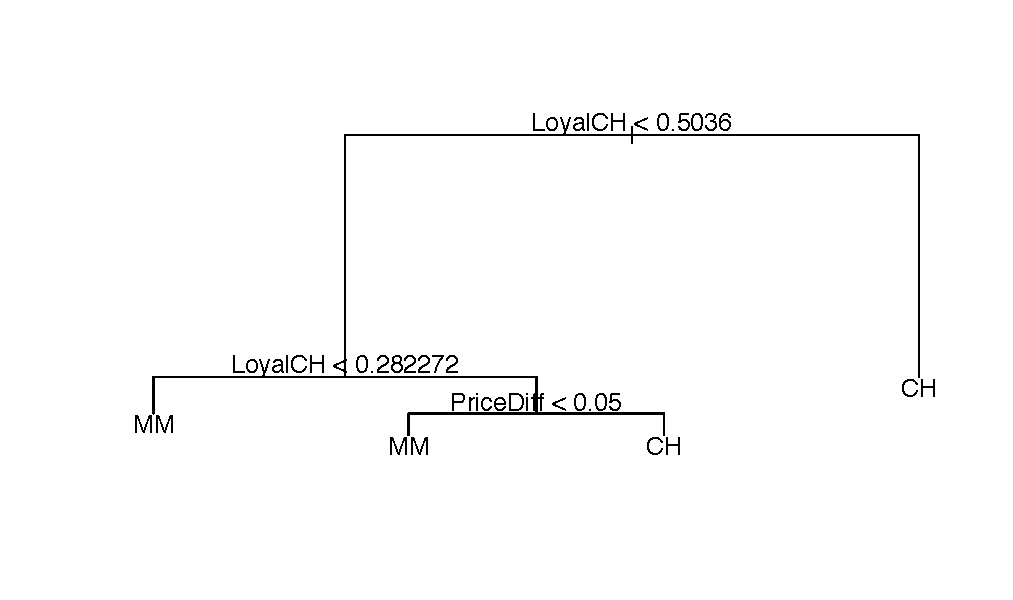
\includegraphics[height=0.35\textheight]{g3.pdf}
\end{center}


\item[\textbf{(j)}] We can obtain the training error for pruned tree:

\begin{lstlisting}
summary(prune.oj)
\end{lstlisting}

\begin{verbatim}
Classification tree:
snip.tree(tree = tree.oj, nodes = c(4L, 10L, 11L, 3L))
Variables actually used in tree construction:
[1] "LoyalCH"   "PriceDiff"
Number of terminal nodes:  4 
Residual mean deviance:  0.9079 = 722.7 / 796 
Misclassification error rate: 0.1825 = 146 / 800 

\end{verbatim}

Compared to the unpruned tree training error rate is 0.1662, the pruned training error rate 0.1825 is higher.

To predict test data using pruned tree:

\begin{lstlisting}
summary(prune.oj)
prune.pred = predict(prune.oj, OJ.test, type="class")
table(prune.pred, OJ.test$Purchase)
\end{lstlisting}

\begin{verbatim}
prune.pred  CH  MM
        CH 155  34
        MM  12  69
        
\end{verbatim}

Calculate the pruned tree test error rate:

\begin{lstlisting}
mean(prune.pred!=OJ.test$Purchase)
\end{lstlisting}

\begin{verbatim}
[1] 0.1703704

\end{verbatim}

The pruned tree test error rate is 0.1703704, compared to the unpruned test error rate 0.1592593, the pruned tree test error rate is higher.

\end{enumerate}


\section*{Problem 2}

For the given logistics curve $\sigma(a)$, $\exists$:

\begin{align*}
\frac{\mathrm{d} \sigma(a)}{\mathrm{d}a} &= \frac{\mathrm{d} }{\mathrm{d}a} \frac{1}{1 + e^{-a}} \\
&= 1 \times \frac{1}{2} \times (1 - \frac{1}{2}) \\
&= \frac{1}{4}
\end{align*}

On the other hand, for the given function $\Phi (a)$, $\exists$:

\begin{align*}
\frac{\mathrm{d} \Phi(\lambda a)}{\mathrm{d}a} &= \frac{\mathrm{d} }{\mathrm{d}a} \int_{- \infty}^{\lambda a} \mathcal{N} (\theta | 0, 1) \mathrm{d} \theta \\
&= \frac{\mathrm{d} }{\mathrm{d}a} \int_{- \infty}^{\lambda a} \left( \frac{1}{\sqrt{2 \pi}} e^{- \frac{\theta^2}{2}} \right) \mathrm{d} \theta \\
&= \frac{\mathrm{d} }{\mathrm{d}a} (\lambda a)  \frac{1}{\sqrt{2 \pi}} e^{- \frac{(\lambda a) ^2}{2}} \\
&= \lambda \frac{1}{\sqrt{2 \pi}} e^{- \frac{(\lambda a) ^2}{2}}
\end{align*}

Two functions are equal at $a=0$, $\exists$:

$$
\lambda \frac{1}{\sqrt{2 \pi}} e^0 = \frac{1}{4}
$$ 

That is 

\begin{align*}
\lambda &= \frac{\sqrt{2 \pi}}{4} \\
\lambda^2 &= \frac{\pi}{8}
\end{align*}

\section*{Problem 3}



Because the Gaussian function in $d$-dimension ($\mathcal{X} = \mathbb{R}^d$) is:

\begin{align*}
\mathcal{N}(\vect{x} | \vect{\mu}, \vect{\varSigma})  = \frac{1}{\sqrt{(2\pi)^d | \vect{\varSigma} |}} \mathrm{exp}{ \left( -\frac{1}{2} (\vect{x}- \vect{\mu})^T \vect{\varSigma}^{-1} (\vect{x} - \vect{\mu}) \right)}\\
\end{align*}

And we have known that $p(t | x, w) = \mathcal{N} ( t | y(x, w), \Sigma)  $,  so the error function ($\log$ form) is:

\begin{align*}
E(\vect{w})
&= \sum_{i=1}^N E_i(\vect{w}) \\
&= \sum_{i=1}^N (- \log p(\vect{t_i} | \vect{x_i}, \vect{w}))\\
&= - \sum_{i=1}^N \log \mathcal{N} (\vect{t_i} | \vect{y(x_i, w)}, \vect{\varSigma}) \\
&=    - \sum_{i=1}^N  \left[   { \left( -\frac{1}{2} (\vect{t_i}- \vect{y(x_i, w)})^T \vect{\varSigma}^{-1} (\vect{t_i} - \vect{y(x_i, w)}) \right)} \log e +  \log \frac{1}{\sqrt{(2\pi)^d | \vect{\varSigma} |}}     \right]\\
&= \frac{1}{2} \sum_{i=1}^N (\vect{t_i}- \vect{y(x_i, w)})^T \vect{\varSigma}^{-1} (\vect{t_i} - \vect{y(x_i, w)}) \log e - \sum_{i=1}^N  \log \frac{1}{\sqrt{(2\pi)^d | \vect{\varSigma} |}}  \\
\end{align*}

Because $\vect{\varSigma}$ is fixed and known, we can clear the error function by removing items irrelevant of $\vect{w}$. The final form of the error function that must be minimized in order to find the maximum likelihood solution for $\vect{w}$ is:

\begin{align*}
E(\vect{w}) = \frac{1}{2} \sum_{i=1}^N (\vect{t_i}- \vect{y(x_i, w)})^T \vect{\varSigma}^{-1} (\vect{t_i} - \vect{y(x_i, w)})
\end{align*}







	


\end{document} 
